%%%%%%%%%%%%%%%%%%%%%%%%%%%%%%%%%%%%%%%%%%%%%%%%%%%%%%%%%%%%%%%%%%%%
% Trello API wrapper
%%%%%%%%%%%%%%%%%%%%%%%%%%%%%%%%%%%%%%%%%%%%%%%%%%%%%%%%%%%%%%%%%%%%
\onehalfspacing
\chapter{Trello API wrapper}\index{Trello}\index{API}\label{apiwrapper}

These scripts fulfill very different tasks, but they have also much in common. For example, almost every script potentially loads single cards. This API wrapper\index{API!wrapper} makes Trello accessible in Ruby\index{Ruby}. Additionally, the scripts can now use the same methods multiple times and, in consequence, they can stay very lightweight and clean. Almost everything that is possible with the Trello API is also possible with this API wrapper. It doesn't cover all features, though, because the API is still in beta phase, so it changes quite quickly.

\begin{figure}
\centering
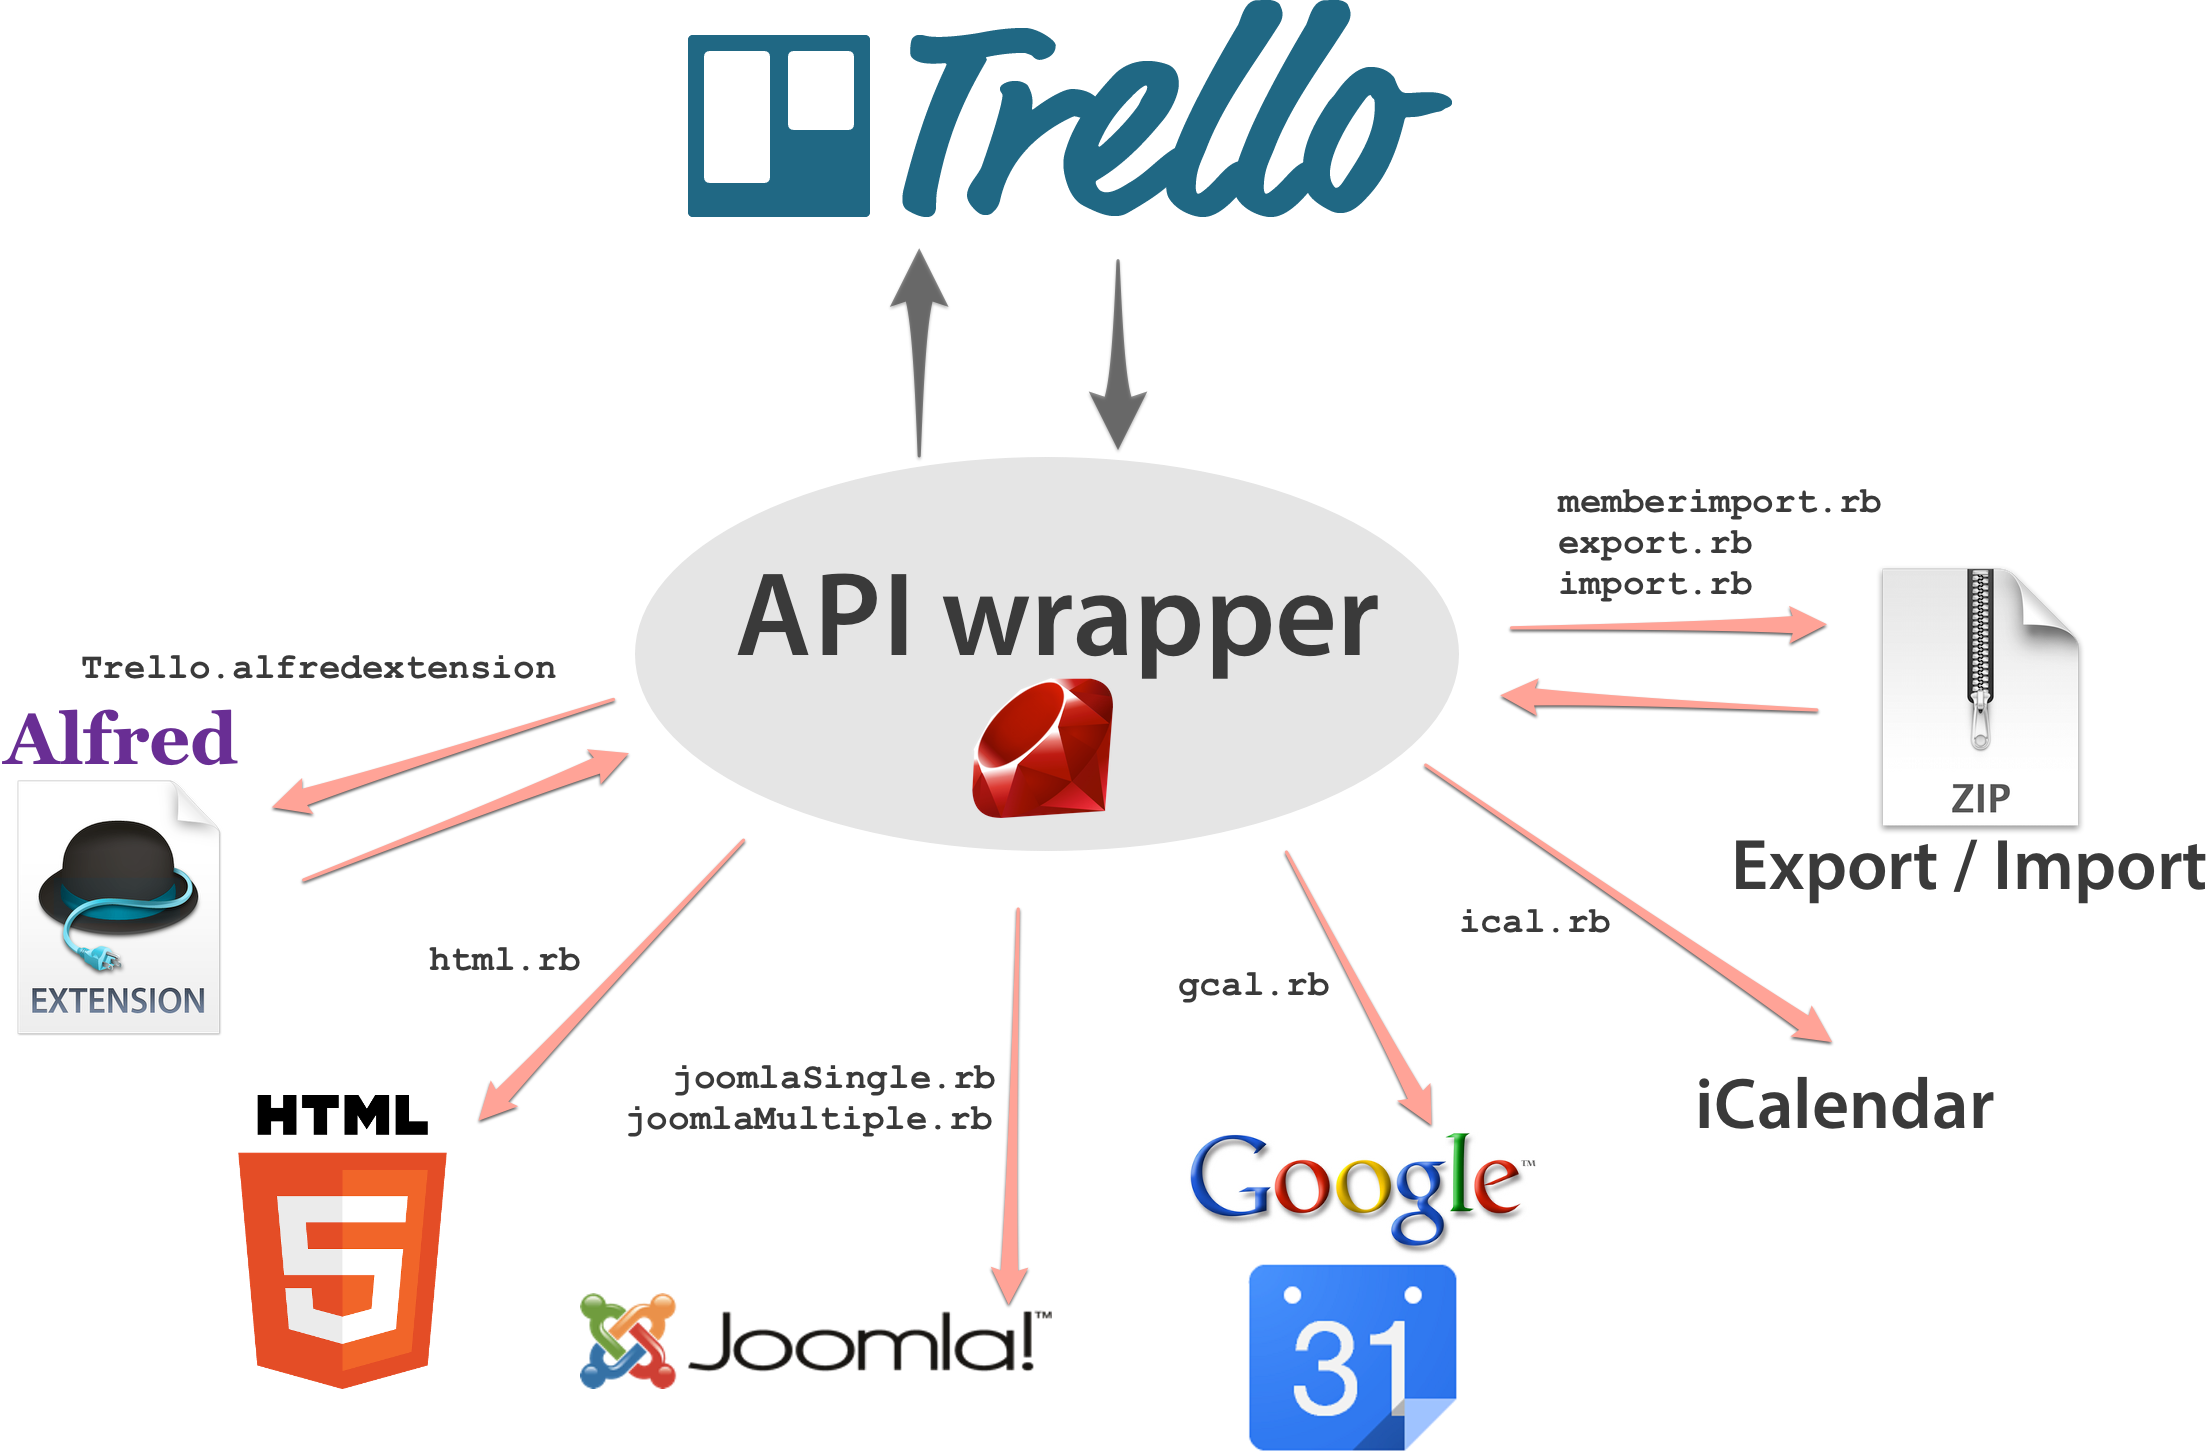
\includegraphics[width=\textwidth]{figures/api-wrapper}
\caption{Connections between Trello, the API wrapper, and the actual features. \cite{ruby:icon}\cite{html:logo}\cite{joomla}\cite{google} }
\label{fig: api-wrapper}
\end{figure}

The API wrapper also has methods to pre-process data for Ruby. From a developer's point of view, Trello is all about cards. Cards are the only things in Trello with real data, not just meta data. So if the task is to get a board from the API\index{API}, it means to get the cards of the board. Although the developer won't be able to read out all information, there is an API call to get all cards belonging in a specific board. So the API wrapper has to execute the API call for a single card to cumulate all the information about all the cards of the board. This is the function of the API wrapper, to keep the actual script clean. So the developer can work with the data and doesn't have to worry about determining it.

The API wrapper is meant to perform all API calls which are required by the scripts. None of the API calls should be performed by the scripts that use the API wrapper.


\section{Command Line Interface}\nomenclature{CLI}{Command Line Interface}\index{CLI}\index{Command-Line Interface}\label{cli}
Almost every script needs some information to run properly. The information which every scripts needs, is the key and token of the user whose account is supposed to be used to access Trello. The scripts have to know which cards, lists, and boards they have to look at. Therefore, this information has to be passed on to the scripts, too. This information could be set at the top of each script. But it is obvious that that it would be very unpractical to hard code this in each script. This way, it would be impossible to use the same Ruby file with several Trello accounts. For every Trello account, the user has to generate a dedicated file. The solution for this problem is a command-line interface (CLI)\index{CLI}. With a CLI, the user can pass on information to the script in a predefined format, so the script knows exactly what to do. For every other call, the user can specify different information for the same script.

The Ruby\index{Ruby} class OptionParser\cite{ruby:optionparser}\index{OptionParser} provides easy customisable command-line option analysis. The developer is able to specify their own options for each script. For this purpose, a dedicated class is used. 
In order to let the actual script \emph{know} about the CLI\index{CLI} arguments, the developer has to require the respective CLI class with the command-line option definitions.

\begin{lstlisting}[aboveskip=1\baselineskip, style=bash, caption=Example usage of a script with CLI., label=listing004]
ruby html.rb -c 4ffd78a2c063afeb066408b8
\end{lstlisting}

An example usage of a script with CLI would look like Listing \ref{listing004}. The \texttt{-c} is a command-line option. If there is a string behind the option, like in this case, the string is a so called \emph{argument}. But there are command-line options which stand by themselves. These are called \emph{flags}, which are for polar decisions only.

\begin{lstlisting}[aboveskip=1\baselineskip, caption=Definition of a command-line option, label=listing002]
# Trello list(s)
opts.on("-l", "--lists x,y,z", Array, "Ids of one or more Trello lists.") do |lists| (*@\label{line001}@*)
	options.lists = lists (*@\label{line300}@*)
end
\end{lstlisting}

Listing \ref{listing002} shows the definition of the option \texttt{-l} for passing one or more IDs of lists to a script. In Line \ref{line001} the word \lstinline{Array} casts the list argument to an Array object.

OptionParse provides an automated help option. If the user types 
\begin{center}
\texttt{ruby script.rb -h} 
\end{center}
they get the explanation the developer wrote in the CLI class for this script with all possible options. This list is automatically generated by the definitions of the command-line options like in Listing \ref{listing002}. It works with \texttt{-help} and \texttt{--help} instead of \texttt{-h}, too.

\begin{lstlisting}[aboveskip=1\baselineskip, style=bash, caption=Output of the \texttt{-h} option., label=listing003]
Usage: ical.rb [options]
Select the input cards with -c, -l, -b or -a

Specific options:
 -a, --[no-]all         Set this if all due dates of all cards of all boards this user can see shall be used.
 -l, --lists x,y,z      Ids of one or more Trello lists.
 -b, --boards x,y,z     Ids of one or more Trello boards.
 -o, --organizations x,y,z Ids of one or more Trello organizations.
 -c, --cards x,y,z      Ids of one or more Trello cards.
 -k MANDATORY, --key    Your Trello key.
 -t MANDATORY, --token  The Trello token.
\end{lstlisting}

Listing \ref{listing003} shows the Output of \texttt{ruby ical.rb -h}. 
These are the basic CLI commands used by every script. For some scripts there are additional commands, which are explained in their respective sections.

All information from the command-line is stored in the \texttt{options} variable. This is an instance of Ruby's\index{Ruby} OpenStruct\index{OpenStruct} class, which is a data structure that allows the definition of random attributes. In line \ref{line300} of listing \ref{listing002} the attribute \texttt{lists} is initialised with a new value. \cite{ruby:openstruct} To read the command-line the script has to instruct the command-line class to parse the command-line arguments considering the specified options. After the command-line is parsed the data in available in a OpenStruct:

\begin{lstlisting}[aboveskip=1\baselineskip, caption=Reading the OpenStruct\index{OpenStruct} containing the command-line information., label=listing046]
options = CLHtml.parse(ARGV)

$key = options.key
$token = options.token
\end{lstlisting}

Listing \ref{listing046} shows how to instruct the corresponding command-line class to parse the command-line information and how to access the data in the OpenStruct. Here the token and key specified in the command-line are provided as global variables to the programme.

\section{Methods}
The API wrapper\index{API!wrapper} contains a huge amount of methods. The API\index{API} calls wrapped by the following methods need a private key and a token to access content in private boards. Thus, private key\index{private key} and token\index{token} need not be sent to each method, it will be initialised in each script as global variables. The variable for the private key\index{private key} is called \lstinline{$key} and the one for the token is called \lstinline{$token}. Global variables\index{variable!global} can be accessed from anywhere within the programme during the runtime.

The methods which wrap a \texttt{GET} or \texttt{DELETE} request look like listing \ref{listing045}. A special URL is visited by the RestClient gem and the response JSON is parsed and returned as hash. 

\begin{lstlisting}[aboveskip=1\baselineskip, caption=\lstinline{getBoardsByMember()}, label=listing045]
def getBoardsByMember(memberId)
	boards = RestClient.get("https://api.trello.com/1/members/"+memberId+"/boards?key="+$key+"&token="+$token+"&filter=open")
	boards = JSON.parse(boards)
end
\end{lstlisting}

The methods which wrap \texttt{POST} or \texttt{PUT} requests look like in listing \ref{listing048}. Several arguments have to or can be passed to the URL. 

\begin{lstlisting}[aboveskip=1\baselineskip, caption=\lstinline{postCard()}, label=listing048]
def postCard(cardName, cardDesc, cardPos, idList)
	response = RestClient.post(
		'https://api.trello.com/1/cards',
		'name' => cardName,
		'desc' => cardDesc,
		'pos' => cardPos,
		'idList' => idList,
		'key'=>$key,
		'token'=>$token
	)
	response = JSON.parse(response)
end
\end{lstlisting}

In this case a new card is created. The Trello API needs the title of the new card, the description, if the card should have one, the position in the list, and the ID of the list it which it should be placed. A example JSON response of a \texttt{POST} request to Trello is shown in listing \ref{listing049}.

\begin{lstlisting}[aboveskip=1\baselineskip, style=bash, caption=JSON response of a \texttt{POST} request., label=listing049]
{"id"=>"504bf790e9e68a282c8b3df6",
 "checkItemStates"=>[],
 "closed"=>false,
 "desc"=>"",
 "idBoard"=>"4ffa4c5ce75c29032a88ea31",
 "idChecklists"=>[],
 "idList"=>"4ffa4c5ce75c29032a88ea32",
 "idMembers"=>[],
 "idShort"=>27,
 "manualCoverAttachment"=>false,
 "labels"=>[],
 "name"=>"Woot!",
 "pos"=>3,
 "url"=>"https://trello.com/card/woot/4ffa4c5ce75c29032a88ea31/27",
 "badges"=>
  {"votes"=>0,
   "viewingMemberVoted"=>false,
   "subscribed"=>false,
   "fogbugz"=>"",
   "checkItems"=>0,
   "checkItemsChecked"=>0,
   "comments"=>0,
   "attachments"=>0,
   "description"=>false,
   "due"=>nil}}
\end{lstlisting}
This JSON\index{JSON} response is parsed to a Ruby hash, as well.

For a documentation on every method of the API wrapper there is a documentation in HTML available.

\subsection{Handling of date and time}
Content in Trello may have set dates. These dates are represented by the Trello API as an ISO\nomenclature{ISO}{International Organization for Standardization} 8601\index{ISO!8601}\footnote{More information about ISO 8601 on the website of the International Organization for Standardization: \url{http://www.iso.org/iso/home/store/catalogue_tc/catalogue_detail.htm?csnumber=40874}. The RFC 3339 is a profile of ISO 8601: \url{http://www.ietf.org/rfc/rfc3339.txt}} formatted string. The timezone\index{timezone} of the date is UTC\nomenclature{UTC}{Universal Time Coordinated}. To ensure that the correct time is always displayed, the date has to be adapted to local time. 

\subsubsection{getDate(date, format='de')}
\begin{lstlisting}[aboveskip=1\baselineskip, caption=\lstinline{getDate()}, label=listing044]
def getDate(date, format='de')
	fdate = Time.iso8601(date).getlocal (*@ \label{line045} @*)
	
	if format=='de'
		return fdate.strftime('%d.%m.%Y %H:%M:%S')
	elsif format=='us'
		return fdate.strftime('%m/%d/%Y %I.%M.%S %P')
	elsif format=='joomla'
		return fdate.strftime('%Y-%m-%d %H:%M:%S')
	elsif format=='ical'
		return fdate.strftime('%Y%m%dT%H%M%S')
	elsif format=='year'
		return fdate.strftime('%Y')
	elsif format=='iso8601'
		return fdate.iso8601
	end
end
\end{lstlisting}

In line \ref{line045} of listing \ref{listing044} the given date string in ISO 8601 format is parsed to a Ruby \lstinline{Time} object. \lstinline{getlocal} is the important part here. This function of the \lstinline{Time} class determines the server's time zone and readjusts the time accordingly. This method respects the daylight saving time\index{daylight saving time} in several time zones\index{time zone}, too. For this method working as intended it is important that the correct time zone\index{time zone} is set on the used server. 

The \lstinline{getDate()} method additionally converts the date to other formats. For example date formats which are required by the iCalendar format or the Joomla CMS.

\subsection{Special methods}
Special methods don't just wrap a Trello API\index{API} call, but accumulate basic information with additional data to get information which the Trello API\index{API} doesn't provide directly.

\subsubsection{getCardsAsArray(arrayCardsStd, downloads = true)}
\begin{lstlisting}[aboveskip=1\baselineskip, caption= getCardsAsArray(), label=listing063]
def getCardsAsArray(arrayCardsStd, downloads = true)
	arrayCardsFull = Array.new
	directoryNameAttachments = File.join(Dir.tmpdir, "attachments")
	
	arrayCardsStd.each do |card|
		# export members
		memberArray = Array.new
		card['idMembers'].each do |memberId|
			member = getMember(memberId)
			memberArray << member			
		end
		membersForCard = Hash.new
		membersForCard['members'] = memberArray
		card = card.merge(membersForCard)
		# end export members		
		
		# export checklists
		hasChecklist = getChecklist(card['id']) 
		
		if hasChecklist[0] != nil
			arrayChecklists = Array.new
			checkItemStates = card['checkItemStates']
			hasChecklist.each do |checklist|  
				hashChecklist = Hash.new  
				hashChecklist['id'] = checklist['id']
				hashChecklist['name'] = checklist['name']
				arrayItems = Array.new
				checklist['checkItems'].each do |item|
					hashItem = Hash.new
					hashItem['name'] = item['name']
					hashItem['completed'] = false
					checkItemStates.each do |state|
						if state.value?(item['id'])
							hashItem['completed'] = true
						end
					end
					hashItem['pos'] = item['pos']
					arrayItems.push(hashItem)
				end
				hashChecklist['items'] = arrayItems
				arrayItems = nil
				arrayChecklists.push(hashChecklist)
				hashChecklist = nil
			end
			
			hashCheckListsForCard = Hash.new
			hashCheckListsForCard['checklists'] = arrayChecklists
			
			card = card.merge(hashCheckListsForCard)
		end
		# end export checklists
		
		# export comments
		if card['badges']['comments'] != 0
			comments = getCardComments(card['id'])
			hashCommentsForCard = Hash.new			
			hashCommentsForCard['commentsContent'] = comments			
			card = card.merge(hashCommentsForCard)
		end
		# end export comments
		
		# export attachments
		if card['badges']['attachments'] != 0
			attachments = getAttachment(card['id'])			
			hashAttachmentsForCard = Hash.new			
			hashAttachmentsForCard['attachments'] = attachments			
			card = card.merge(hashAttachmentsForCard)			
			
			if downloads
				# download files
				attachments.each do |attachment|
					fileDomain = URI.parse(attachment['url']).host
					filePath = attachment['url'].gsub(URI.parse(attachment['url']).scheme+"://"+URI.parse(attachment['url']).host, '')
					fileExtension = File.extname(attachment['url'])
					
					fileName = attachment['id']+File.basename(attachment['url'])
					puts "Downloading \'"+fileName+"\'"
								
					if !Dir.exists?(directoryNameAttachments)
						Dir::mkdir(directoryNameAttachments)
					end
					
					Net::HTTP.start(fileDomain) do |http|
							resp = http.get(filePath)
							open(directoryNameAttachments+"/"+fileName, "wb") do |file|
									file.write(resp.body)
							end
					end      
				end
				# download files
			end       
		end	
		# end export attachments
		
		# export votes
		if card['badges']['votes'] > 0
			response = RestClient.get(
					'https://api.trello.com/1/cards/'+card['id']+'/membersVoted?key='+$key+'&token='+$token
			)
			members = JSON.parse(response)
			membersVotedArray = Array.new
			members.each do |member|
				 membersVotedArray.push(member['id'])
			end
			hashMembersVotedForCard = Hash.new			
			hashMembersVotedForCard['membersVoted'] = membersVotedArray
			card = card.merge(hashMembersVotedForCard)	
		end
		# end export votes
		
		arrayCardsFull.push(card)
	end
	
	return arrayCardsFull
end
\end{lstlisting}

The \lstinline{getCardsAsArray()} method is one of the biggest methods of the API wrapper\index{API!wrapper}. The methods to get all cards of a board or a list don't provide all information of the cards. If those functions don't supply all data which is needed for a specific task the missing information has to be added. That is what \lstinline{getCardsAsArray()} is doing. The method is provided with an array of cards. Then it accumulates all information about all cards in this array. That includes members which are assigned to a card, checklists and according check items of a card, comments, attachments and votes. The developer can decide if attachments should be downloaded to a directory in the temporary directory of the operating system. In order to complete that task the method has to iterate through all cards and execute specific API\index{API} calls to get the required information from Trello. Those API calls are wrapped in other methods which are structured like the method in listing \ref{listing045}. The return value of \lstinline{getCardsAsArray()} is an array with the whole information about the required cards.


\subsubsection{isThisMe(memberId)}
\begin{lstlisting}[aboveskip=1\baselineskip, caption= isThisMe(), label=listing059]
def isThisMe(memberId)
	if getMember('me')['id'] == memberId
		return true
	else
		return false
	end
end
\end{lstlisting}

The \lstinline{isThisMe()} method can be used to check if some content of a backup belonged to the actually used Trello account. For example to get all own comments out of an older backup.

\subsection{Accessing CMS}
To access CMS\index{CMS} there are two methods. \lstinline{trelloToJoomlaSingle(joomlaArticleId, articles)} and \lstinline{trelloJoomlaSync(cardId, sectionid, catid, joomlaVersion)}. These are both to write data into the database\index{databse} of the Joomla\index{Joomla} CMS\index{CMS}.


\subsubsection{trelloJoomlaSync(cardId, sectionid, catid, joomlaVersion)}

\begin{lstlisting}[aboveskip=1\baselineskip, caption=Getting standard card information., label=listing029]
card = getSingleCard(cardId)
title = card['name']  (*@ \label{line025}@*)
description = Kramdown::Document.new(card['desc']).to_html  (*@ \label{line026}@*)
\end{lstlisting}

\lstinline{trelloJoomlaSync()} must determine a card's whole information itself. The \lstinline{getSingleCard()} supplies the standard information of a card such as the title in line \ref{line025} of listing \ref{listing029} and the description in line \ref{line026}. Again, the \texttt{kramdown} gem is used to convert the Markdown\index{Markdown} formatted description string to HTML\index{HTML}. But attachments and checklists would also be meaningful to depict in a CMS\index{CMS}. Besides, the cards creation or update date is required to decide whether a card has changed or not.

\begin{lstlisting}[aboveskip=1\baselineskip, caption=Getting the date of a cards last change., label=listing030]
changed = nil
if !cardUpdated(cardId).empty?
	changed = getDate(cardUpdated(cardId).first['date'], 'joomla')
else
	changed = getDate(cardCreated(cardId).first['date'], 'joomla')
end
\end{lstlisting}
There is an API call for the last update of a card. But if the card has never been updated, the response would be empty. So in this case, the API call for the creation date must be used.

\begin{lstlisting}[aboveskip=1\baselineskip, caption=Processing the attachments of a card., label=listing031]
hasAttachment = getAttachment(cardId) (*@ \label{line027}@*)

if hasAttachment[0] != nil
	description += "<ul>"		
	hasAttachment.each do |att|	
		description += "<li><a href=\""+att['url']+"\">\""+att['name']+"\"</a></li>"
	end
	description += "</ul>"
end
\end{lstlisting}

To get the attachments of a card, the \lstinline{getAttachment(cardId)} method is used in line \ref{line027} of listing \ref{listing031}. If the API\index{API} call contains attachment data, the HTML\index{HTML} tag \lstinline{<ul>} is appended to the description. After that, the attachments are appended as list items. Their names are simply linked with the URL\index{URL} to the file on Trello's servers. 

\begin{lstlisting}[aboveskip=1\baselineskip, caption=Processing the checklists of a card., label=listing032]
hasChecklist = getChecklist(cardId) 

if hasChecklist[0] != nil
	hasChecklist.each do |checklist| 			
		description += "<h4>"+checklist['name']+"</h4>"
		description += "<ul>"
		checklist['checkItems'].each do |item|	
			if isCompleted(cardId, item['id'])
				description += "<li><del>"+item['name']+"</del></li>"
			else
				description += "<li>"+item['name']+"</li>"
			end
		end
		description += "</ul>"
	end	
end
\end{lstlisting}

To process the checklists of a card, the method \lstinline{getChecklist(cardId)} is called first. If the response contains checklist data, a \lstinline{<h4>} HTML tag with the checklist's name is added to the description. After that, another \lstinline{<ul>} is started. The \lstinline{isCompleted()} method must be called for every checklist item to resolve its status. In dependency of the result, the name of the item is displayed as crossed out or not. Ruby's\index{Ruby} append method is used because the description already is a HTML\index{HTML} string.

Now, that the content is available to the script, it must be written to the database. Because the \lstinline{trelloJoomlaSync()} method supports Joomla\index{Joomla} versions 1.5 and 2.5, every database query exists twice. From Joomla 1.5 to Joomla\index{Joomla} 2.5, the underlying database\index{database} structure has changed a bit. 

\begin{lstlisting}[aboveskip=1\baselineskip, caption=\texttt{joomlaMultiple.rb} usage., label=listing033]
begin  
	existingArticleQuery = my.query(" (*@ \label{line028}@*)
		SELECT id, created, modified
		FROM jos_content 
		WHERE metadata='"+cardId+"'
	") (*@ \label{line029}@*)
rescue Mysql::Error => e
	puts e
else
	# if article doesn't exist insert it into the db
	if existingArticleQuery.num_rows == 0
		begin
			
			# Insert new article, see listing (*@ \ref{listing034} @*)(*@ \label{line030}@*)
			
		rescue Mysql::Error => e
			puts e
			return
		ensure
			stmt.close if stmt
		end			
	else
		# this should be only one because per Trello card ID should only exist one article in Joomla
		existingArticleQuery.each do |thisArticle|
			
			existingId = thisArticle[0]
			existingCreated = thisArticle[1]
			existingModified = thisArticle[2]
			
			# check if the modified timestamp im Trello is different to the modified timestamp in Joomla
			begin 
				if existingModified != changed
					
					# Update article, see listing (*@ \ref{listing036} @*)(*@ \label{line032}@*)
					
					puts 'Changed: '+cardId+" : "+title
				else 
					puts 'Nothing changed: '+cardId+" : "+title
				end					
			rescue Mysql::Error => e
				puts e
				return
			ensure
				stmt.close if stmt
			end
		end
	end	
ensure
	my.close if my
end
\end{lstlisting}

In the first \lstinline{begin} block of listing \ref{listing033}, from line \ref{line028} to line \ref{line029}, the method scans the database table \lstinline{jos_content} for an article with the actual handled card ID in the \lstinline{metadata} field. If the response of this query is an empty array, the card isn't in the database. The script then must insert a new article into the database\index{database}. This is performed in line \ref{line030}. The corresponding MySQL\index{MySQL} code is showed in listing \ref{listing034}. If the resulting array in line \ref{line028} contains a row, the script must check if the new data is more recent than the data in the database. This array cannot contain more than one row because the script inserts the article just once if it is new, otherwise it replaces the old article with an updated version. In order to do that, the script looks at the \lstinline{modified} field of the existing article. This date is saved in the \lstinline{existingModified} variable. The update date of the actual Trello card, which is determined in listing \ref{listing030}, is stored in the \lstinline{changed} variable. If \lstinline{existingModified} differs from \lstinline{changed}, the article is updated with the new date of the Trello card in line \ref{line032}. The script assumes that the Trello card always contains correct data. So it's not necessary to check back if the \lstinline{changed} is actually more recent. The MySQL statement\index{MySQL!statement} of the update statement is showed in listing \ref{listing036}.

\begin{lstlisting}[aboveskip=1\baselineskip, caption=Insert new article in the Joomla database., label=listing034]
begin
	stmt = my.prepare("
		INSERT INTO jos_content (
			title, 
			alias, 
			`introtext`, 
			state, 
			sectionid, 
			catid, 
			created, 
			created_by, 
			modified,
			parentid, 
			ordering, 
			access,					
			metadata
		)
		VALUES (
			?, 
			?, 
			?, 
			1, 
			?, 
			?, 
			?, 
			62, 
			?,
			0, 
			1, 
			0,
			?
		)
	")
	
	stmt.execute title, title.downcase, description.gsub((*@/'/@*), '&(*@\#@*)39;'), sectionid, catid, changed, changed, cardId
	puts 'New article: '+cardId+" : "+title
rescue Mysql::Error => e
	puts e
	return
ensure
	stmt.close if stmt
end
\end{lstlisting}


\begin{lstlisting}[aboveskip=1\baselineskip, caption=Updating existing Joomla article., label=listing036]
stmt = my.prepare("
	UPDATE jos_content 
	SET
		title = '"+title+"',
		alias = '"+title.downcase+"',
		`introtext` = '"+description.gsub(/'/, '&#39;')+"',
		state = 1,
		sectionid = 5,
		catid = 34,
		created = '"+changed+"',
		created_by = 62,
		modified = '"+changed+"',
		parentid = 0,
		ordering = 1,
		access = 0
	WHERE
		metadata = '"+cardId+"'
")
stmt.execute
\end{lstlisting}

\subsubsection{trelloToJoomlaSingle(joomlaArticleId, articles)}

\lstinline{trelloToJoomlaSingle()} works like \lstinline{trelloJoomlaSync()}, but it writes all information in Joomla\index{Joomla} in one single article and in HTML\index{HTML} format.

\begin{lstlisting}[aboveskip=1\baselineskip, caption= trelloToJoomlaSingle(), label=listing061]
def trelloToJoomlaSingle(joomlaArticleId, articles)
	# Database connection
	dbhost = 'host'
	dbuser = 'user'
	dbpassword = 'password'
	db = 'dbname'
	
	htmlSite = "<h3>Universit&auml;t T&uuml;bingen</h3>"
	
	htmlSite << "<p> </p>
	<table style=\"text-align: center;\" border=\"0\">
	<tbody>
	<tr style=\"background-color: #c3d2e5;\">
	<td style=\"text-align: center;\">
	<p style=\"text-align: left; padding-left: 5px;\"><strong><span><strong> Thema</strong></span></strong></p>
	</td>
	</tr>"
	
	i = 0
	articles.each do |element|
		title = element.title
		description = element.description
		if element.attachments != []		
			attachments = element.attachments
		end
		
		htmlSite << "
		<tr style=\"background-color: "
		if i.even? 
			htmlSite << "#e0e8ec;"
		else
			htmlSite <<"#c3d2e5"
		end
		htmlSite << "\">
		<td><p style=\"text-align: left; padding-left: 5px;\"><span><strong>"
		htmlSite << title
		htmlSite << "</strong></span></p>
		<div style=\"text-align: left; padding-left: 5px;\"><span style=\"font-size: xx-small;\">"
		htmlSite << description		
		htmlSite << "</span></div>
		<div style=\"text-align: left;\"><span style=\"font-weight: normal; font-size: small;\"> 
		<ul>"
		if element.attachments != []
			attachments.each do |attachment|
				name = attachment.name
				url = attachment.url
				htmlSite << "<li><a href=\""
				htmlSite << url
				htmlSite << "\">"
				htmlSite << name
				htmlSite << "<a/></li>"
			end	
		end	
		htmlSite << "</ul>
		</span></div>
		</td>
		</tr>"	
		i += 1
	end
	i = nil
	
	htmlSite << "</tbody>
	</table>"
	
	#save to file	
	fileHtml = File.new("arbeiten.html.tmp", "w+")
	fileHtml.puts "<!doctype html>
	<head>
		<meta charset=\"UTF-8\">
		<meta http-equiv=\"X-UA-Compatible\" content=\"IE=edge,chrome=1\">
	
		<title>Abgeschlossene Arbeiten</title>
	</head>
	<body>"
	fileHtml.puts htmlSite	
	fileHtml.puts "</body></html>"
	File.rename("arbeiten.html.tmp", "arbeiten.html")
	
	#save to DB
	my = Mysql.init
	my.options(Mysql::SET_CHARSET_NAME, 'utf8')
	my.real_connect(dbhost, dbuser, dbpassword, db)
	my.query("SET NAMES utf8")

	stmt = my.prepare("UPDATE jos_content SET `introtext`='"+htmlSite+"' WHERE id="+joomlaArticleId.to_s)
	stmt.execute
	
	my.close if my
	
end
\end{lstlisting}










